\chapter{Анализ результатов\label{chapter_2}}
\section{Особенности реализации}

При реализации методов, описанных в предыдущем пункте использовался язык C++, стандарт 2011 года.
Структура проекта была разбита на несколько составных частей:
\begin{itemize}
\item[1.] Описание численного метода Симпсона.
\item[2.] Описание численного метода Гаусса.
\item[3.] Описание граничных условий.
\item[4.] Описание самого процесса деформирования.
\end{itemize}

В первых двух пунктах был применена технология шаблонов, так как к функциям интегрирования обращаются объекты разных классов.
Шаблон(template)~--- средство языка C++, предназначенное для кодирования обобщённых алгоритмов, без привязки к некоторым параметрам (например, типам данных, размерам буферов, значениям по умолчанию). В C++ возможно создание шаблонов функций и классов.

В частности были написаны обобщенные функции интегрирования методом Гаусса и методом Симпсона, которые на вход принимали объект, у которого присутствовал оператор, вычисляющий значение подынтегральной функции, а тип объекта определен не был, так в эти функции передавались объекты различных классов. 

В стандарте C++11 появилась встроенная поддержка многопоточности, что также было использовано в работе.
Потоком в программировании называют легковесный процесс, имеющий с процессом-родителем общие ресурсы, такие как память, тогда как процессы не разделяют этих ресурсов. В частности, потоки разделяют инструкции процесса (его код) и его контекст (значения переменных, которые они имеют в любой момент времени).

Задача о деформировании мембраны внутри криволинейной матрицы связана с большим количеством вычислений интегралов. Алгоритм вычисления интеграла с неопределенным верхним пределом выглядит так:
\begin{itemize}
\item разбиваем область верхнего предела на отдельные участки;
\item вычисляем по каждому участку значение;
\item суммируем полученный результат, получая непрерывные значения.
\end{itemize}
		\begin{figure}[h!]
				\center{\includegraphics[width=0.7\linewidth]{images/img4.jpg}}
				\caption{ Время работы программы } 
				\label{parall_results}
	    \end{figure}

Как видно из алгоритма, второй пункт можно вычислять независимо для каждого интеграла. В результате разбиения задач по потокам для свободного и стесненного деформирования внутри криволинейной матрицы было получено ускорение отображаемое на рис.\ref{parall_results}. Отметим, что во второй задаче, где фигурирует матрица с вертикальными стенками и плоским днищем, результаты распараллеливания не приведены, так как там слишком малое время вычисления из-за упрощенных формул для вычисления толщины мембраны на каждом шаге, в силу вида матрицы.

Для представления двух типов графических данных требуется разный формат вывода основного вычислительного ядра системы.
Рассмотрим общую схему программного комплекса, разработанного в рамках данной работы (рис.\ref{programm}).
\begin{figure}[h!]  	
				\def\svgwidth{\columnwidth}
				\center{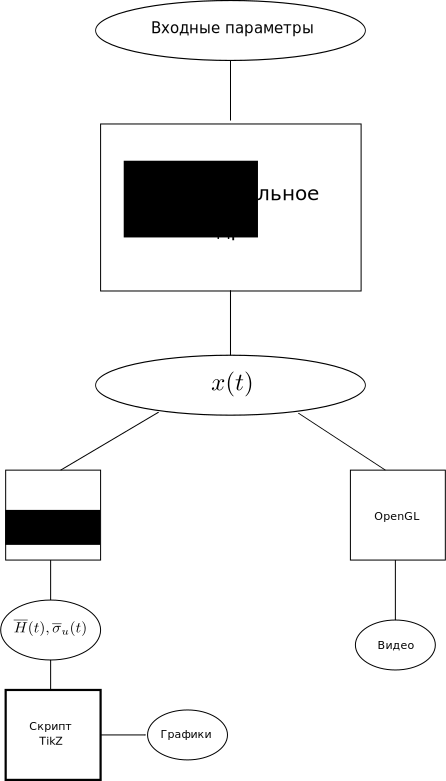
\includegraphics[width=0.8\linewidth]{images/programm.pdf}}
			\caption{ Программный комплекс } 
\label{programm}
 \end{figure}
 
 Для получения качественных графических представлений зависимостей использовался пакет TikZ[\ref{tikz-manual}],
 позволяющий получать качественное векторное представление расчетных данных. 
 Вычислительное ядро может работать в двух режимах: на вовод данных для анимирования, о которых будет рассказано в пункте 3 этой главы, и на вывод данных для построения графиков. Эти данные конвертируются подпрограммой в представление зависимостей основных характеристик деформирования от времени, а затем, полученные данные, поступают на вход скрипту TikZ, строящему по этим данных графики, представленные в пункте 2 текущей главы (рис.\ref{quad_sliging} - \ref{vert_stick_10ba}).
 %мб. что-нить пр тикз написать? кто его создал и вообще что есть такой замечательный инструмент)))
 
\section{Анализ численного эксперимента\label{section_2}}
\subsection{Деформирование внутри криволинейной матрицы}
	В качестве примера рассмотрим деформирование мембраны из алюминиевого сплава Д16T при $400^\circ\text{C}$ [\ref{teraud}]. Константы материала: 
   $C=9.37\cdot10^5 \text{МПа}^{-n}\text{сек}^{-1}$, $n=3.4$, $\sigma_b = 88.3\; \text{МПа}$. 
   Геометрические размеры мембраны: ширина $2a=200$ мм, толщина $H_0=2$ мм, $k$=1.5, $\overline{b}$=4.5 давление $q=2.65$ кПа [\ref{teraud}].  
   
   Вычисления показали, что мембрана в условиях идеального скольжения полностью заполняет криволинейную матрицу $y=4.5(1-x^{1.5})$ за бесконечное время. 
   Стадия мгновенного деформирования характеризуется параметром $\overline{H}_1 = 0.97$, 
   стадия свободного деформирования характеризуется параметрами $\overline{H}_2 = 0.69, \overline{t}_2 = 5.36 \cdot 10^8$.
   На рис.\ref{quad_sliging} представлен график зависимости толщины мембраны и интенсивности напряжения от времени
   (кривые 1 и 2 соответственно).
   
   		\begin{figure}[h!]	
				\def\svgwidth{\columnwidth}
				\center{\includegraphics[width=0.9\linewidth]{images/quad_sliding.png}}
				\caption{Зависимости толщины(1) и интенсивности напряжений(2) от времени при условии идеального скольжения внутри криволинейной матрицы.} 
				\label{quad_sliging}
		\end{figure}

Расчет для прилипания, как граничного условия,	показал, что для начальных данных, идентичных случаю скольжения 
	мембрана разрушается при толщине $\overline{H}=0.015$ за время $\overline{t}=12.15\cdot 10^8$, достигая предельно допустимого напряжения $\sigma_b$.    На рис.\ref{quad_sticking} представлен график зависимости толщины мембраны и интенсивности напряжения от времени (кривые 1 и 2 соответственно).
   
		\begin{figure}[h!]	
				\def\svgwidth{\columnwidth}
				\center{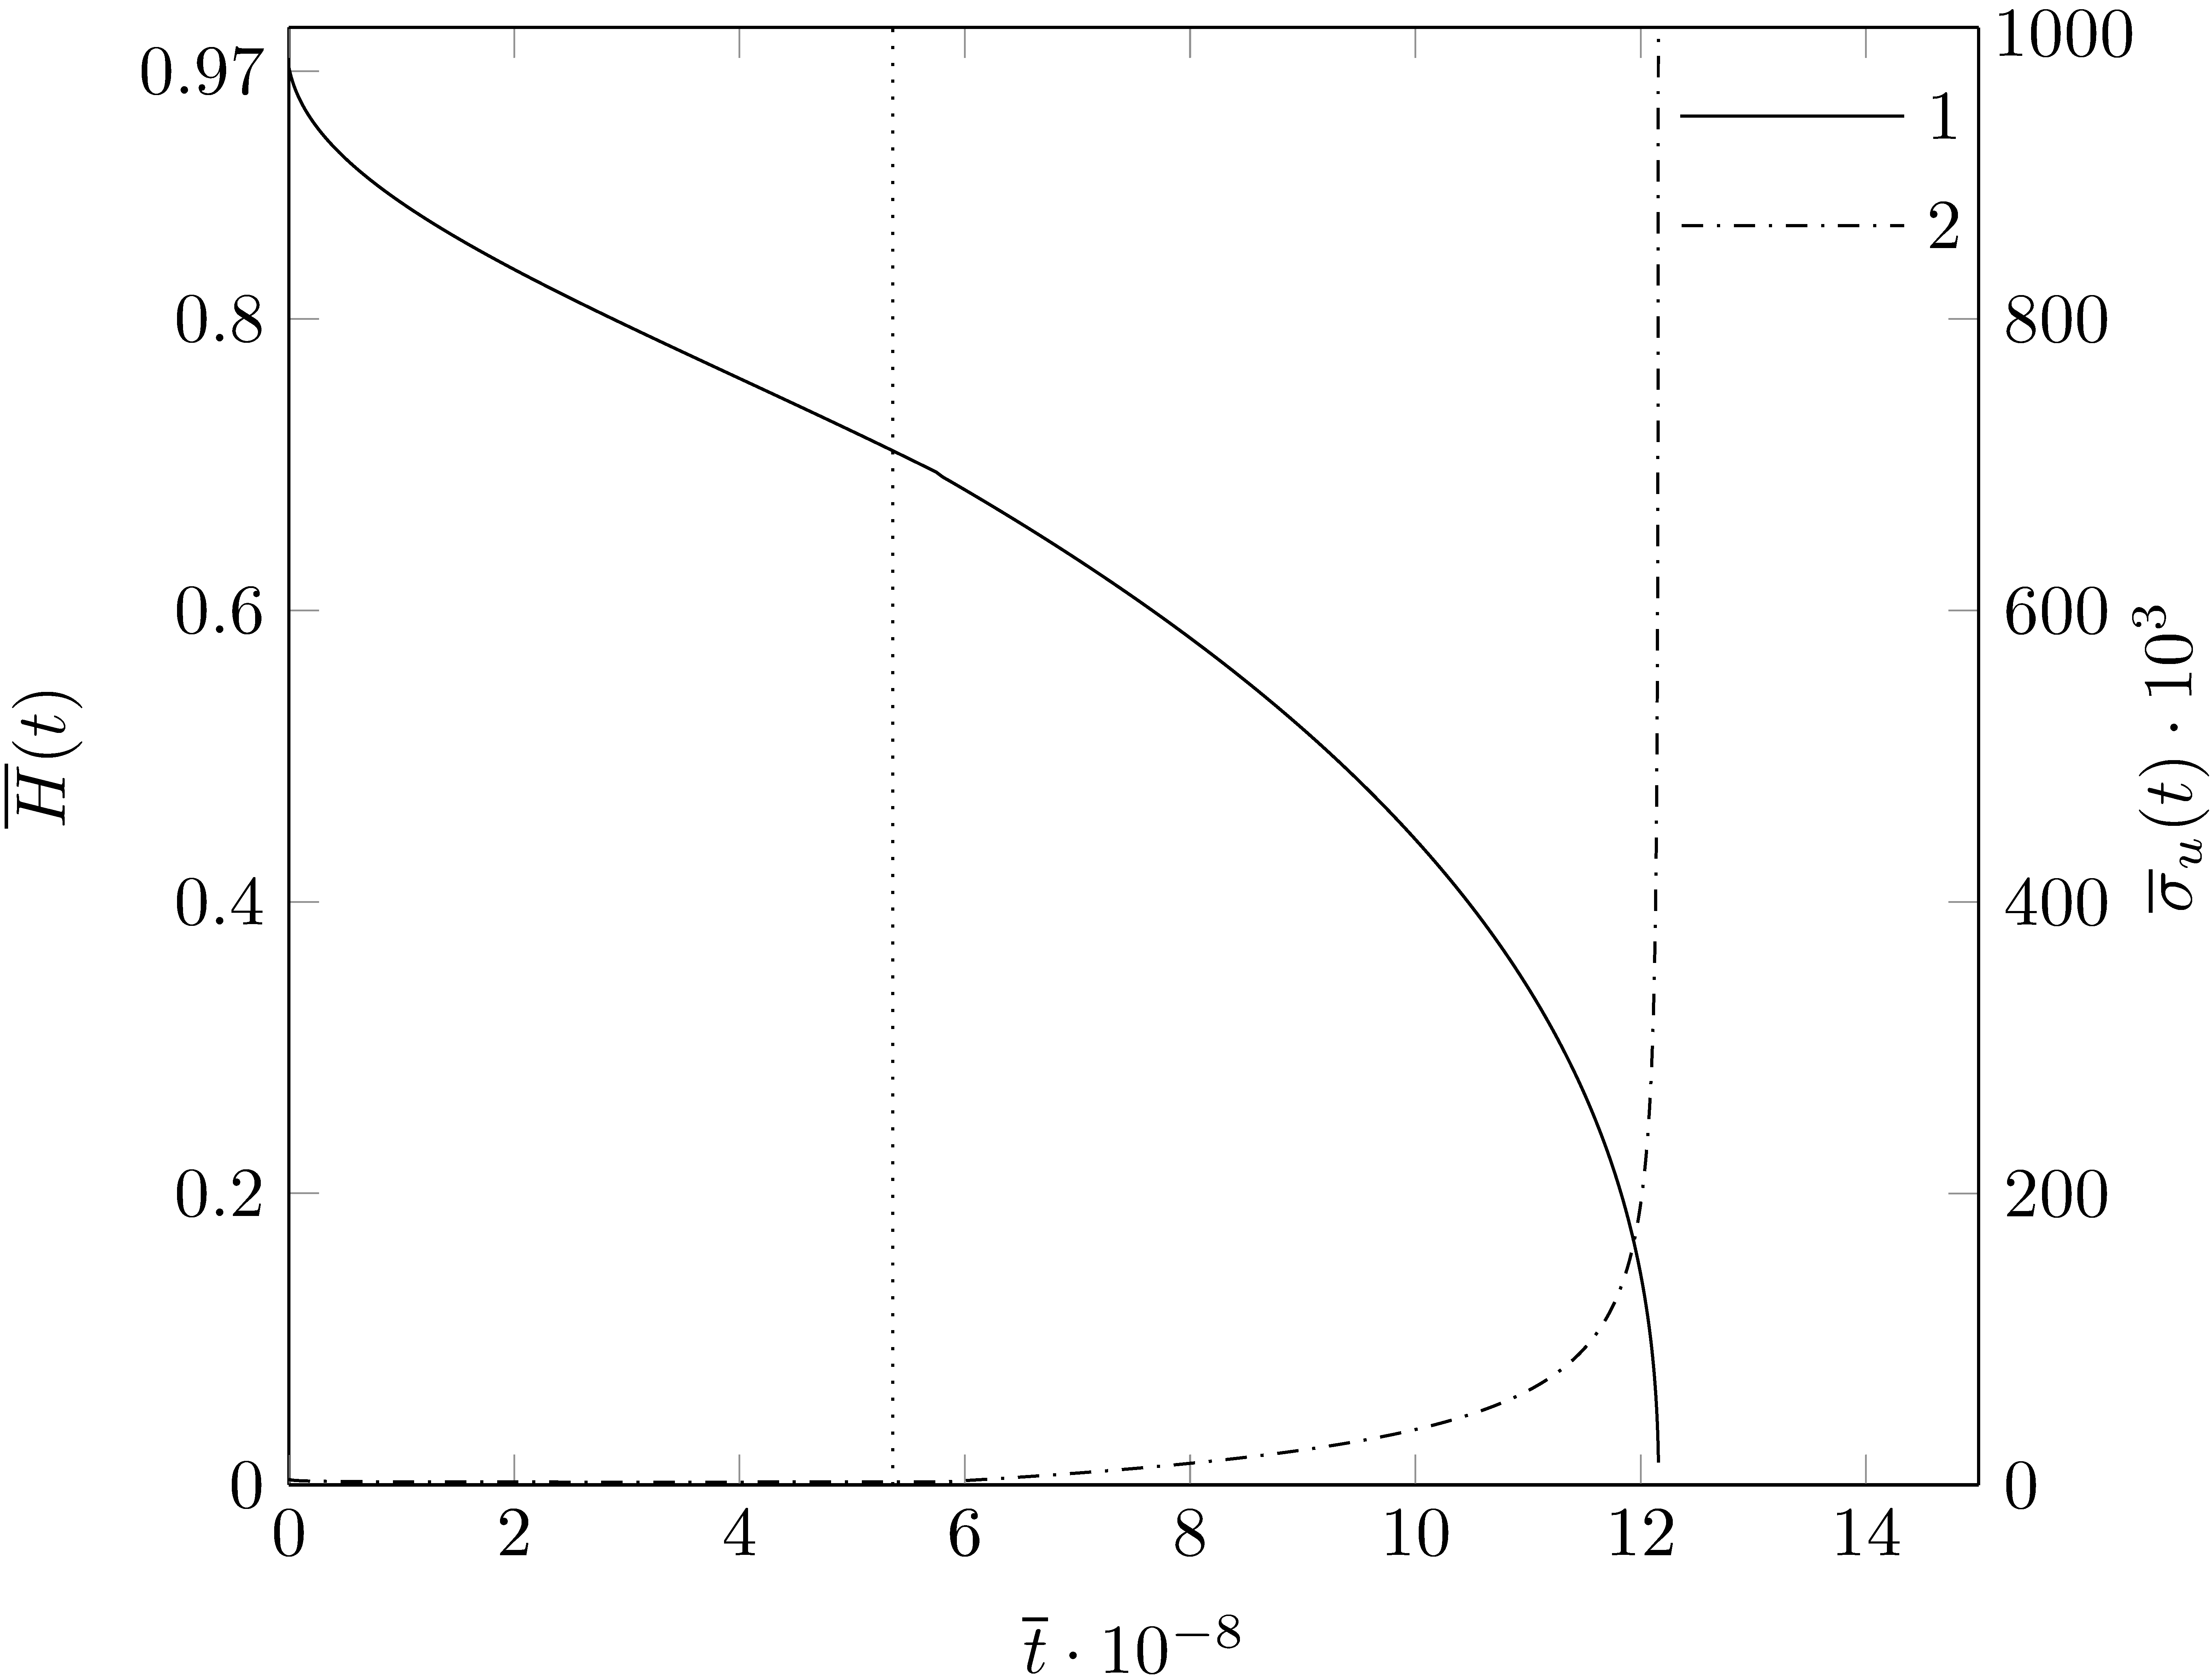
\includegraphics[width=0.9\linewidth]{images/quad_sticking.png}}
				\caption{Зависимости толщины(1) и интенсивности напряжений(2) от времени при условии прилипания внутри криволинейной матрицы. } 
				\label{quad_sticking}
		\end{figure}

\subsection{Деформирование внутри матрицы с вертикальными стенками и плоским днищем}
		
		Расчет для мембраны внутри матрицы с вертикальными стенками и плоским днищем проводился для матриц с различной высотой:
		$b = a$ (рис.\ref{vert_sliging_ba}), $b = 4.5a$ (рис.\ref{vert_sliging_4ba}),$b=7a$ (рис.\ref{vert_sliging_7ba}), $b=10a$ (рис.\ref{vert_sliging_10ba}). Из рисунков видно, что при увеличении высоты мембраны увеличивается максимально достижимая интенсивность напряжения, которая при достижении значения $\sigma_b$ приведет к разрушению мембраны. Приведем результаты вычислений в таблице 1.
\begin{table}
\begin{center}

\renewcommand{\arraystretch}{2}

\begin{tabular}{|c|c|c|}
\hline
$b/a$    & $\overline{t_2}$/$\overline{H_2}$ & $\overline{t_3}$/$\overline{H_3}$ \\
\hline\hline
1    & $7.14\cdot10^8$/0.636  & $7.14\cdot10^8$/0.636\\ \hline
4.5  & $7.14\cdot10^8$/0.636  & $13.67\cdot10^8$/0.186\\ \hline
7    & $7.14\cdot10^8$/0.636  & $13.96\cdot10^8$/0.125\\ \hline
10   & $7.14\cdot10^8$/0.636  & $13.98\cdot10^8$/0.089\\ \hline
\end{tabular}

\end{center}
\label{vert_table}
\caption{}
\end{table}				 
		\begin{figure}[h!]	
				\def\svgwidth{\columnwidth}
				\center{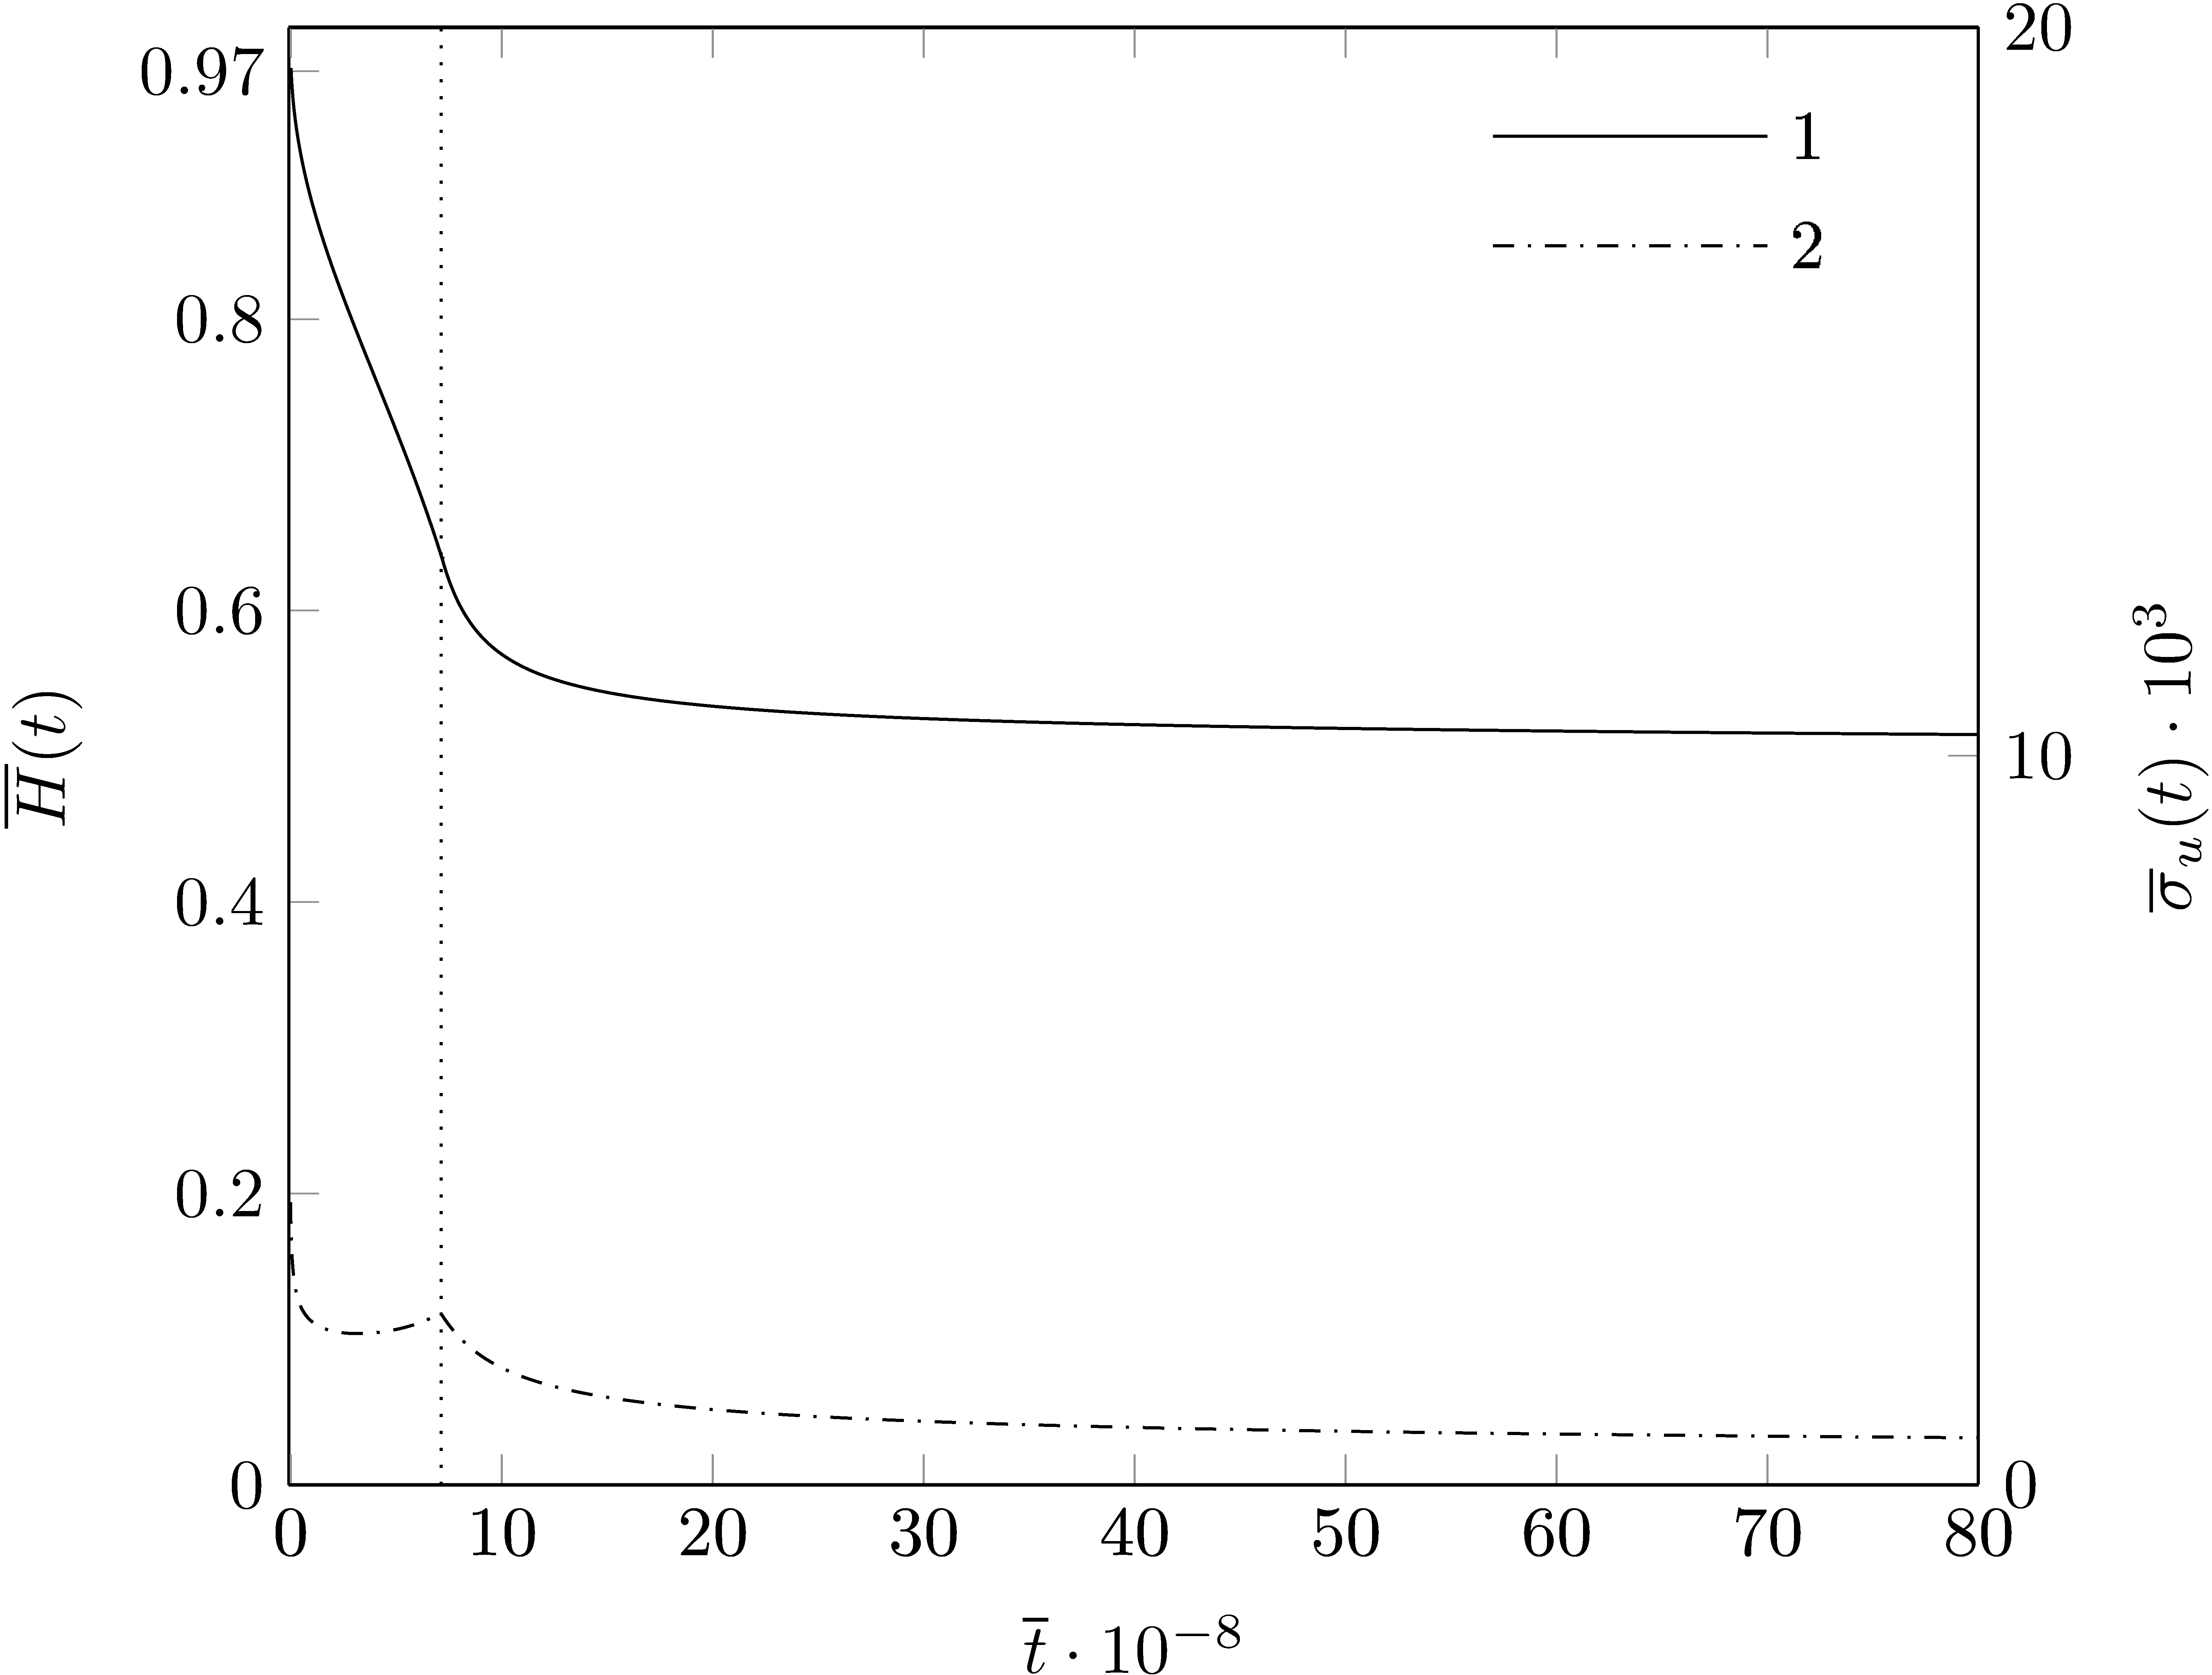
\includegraphics[width=0.8\linewidth]{images/ab.png}}
				\caption{Зависимости толщины(1) и интенсивности напряжений(2) от времени при условии идеального скольжения внутри П-образной матрицы. Отношение $b/a = 1$} 
				\label{vert_sliging_ba}
		\end{figure}

		\begin{figure}[h!]	
				\def\svgwidth{\columnwidth}
				\center{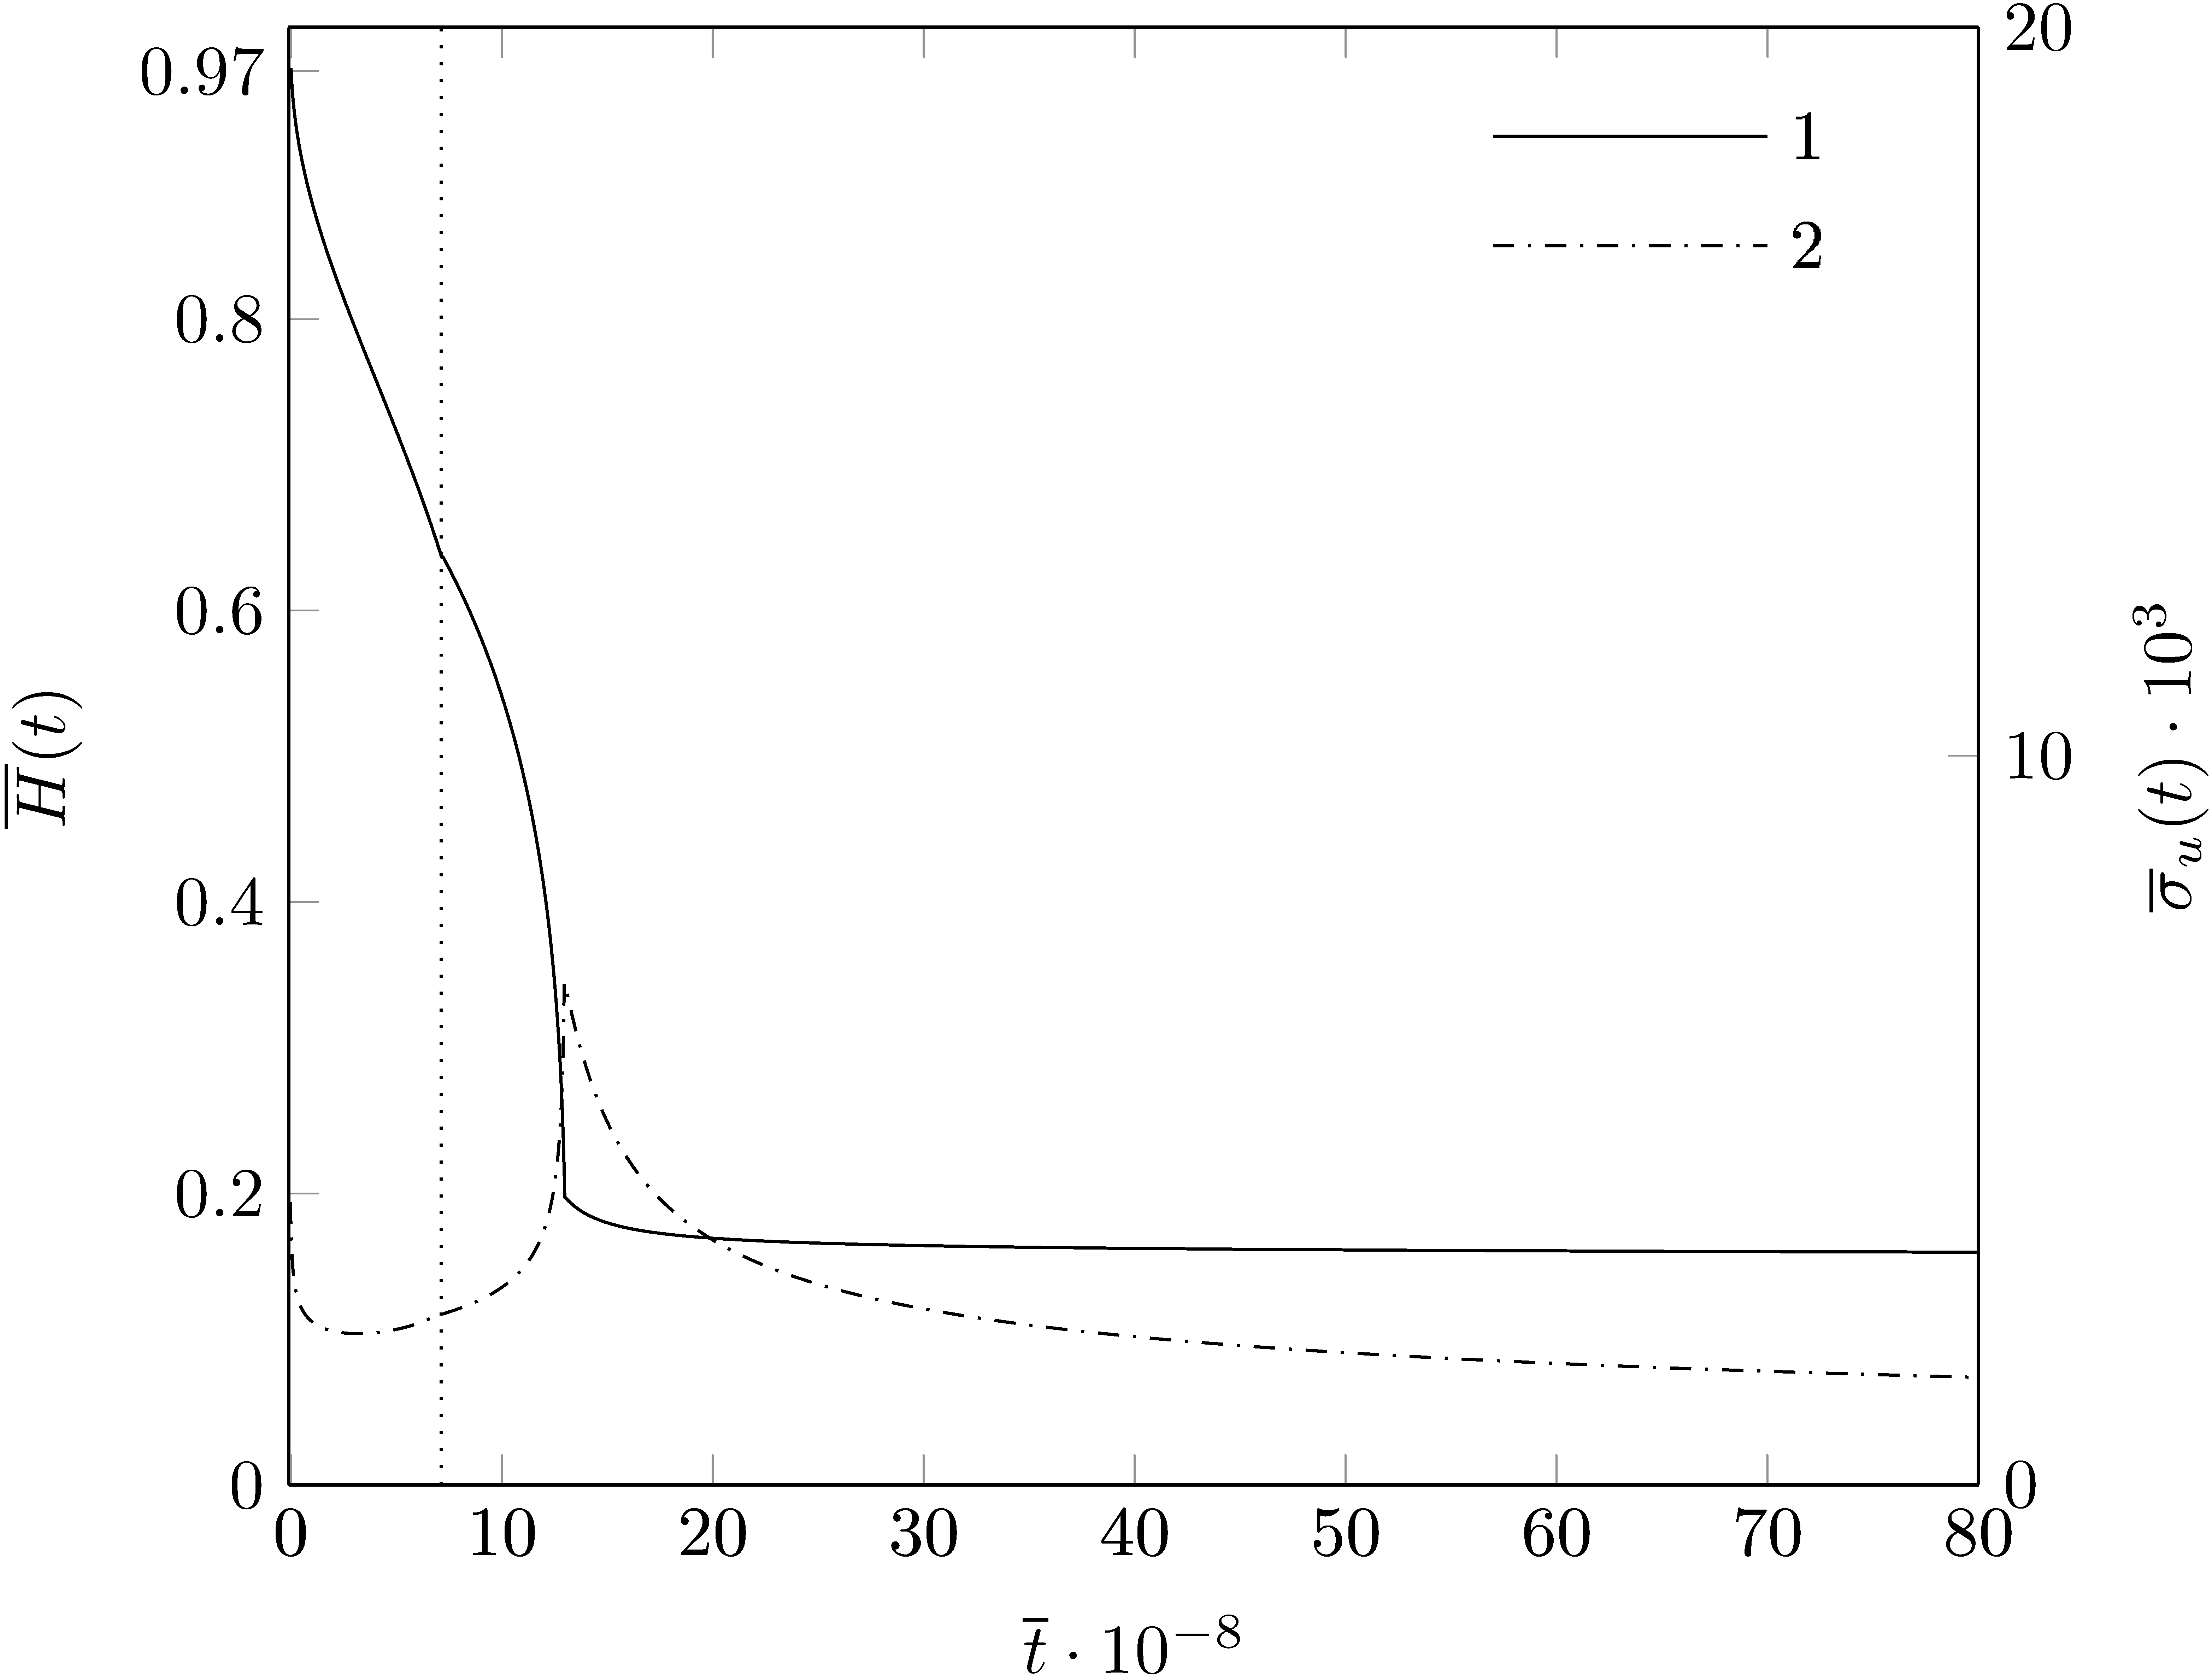
\includegraphics[width=0.8\linewidth]{images/ab4.png}}
				\caption{Зависимости толщины(1) и интенсивности напряжений(2) от времени при условии идеального скольжения внутри П-образной матрицы. Отношение $b/a = 4.5$} 
				\label{vert_sliging_4ba}
		\end{figure}
				\begin{figure}[h!]	
				\def\svgwidth{\columnwidth}
				\center{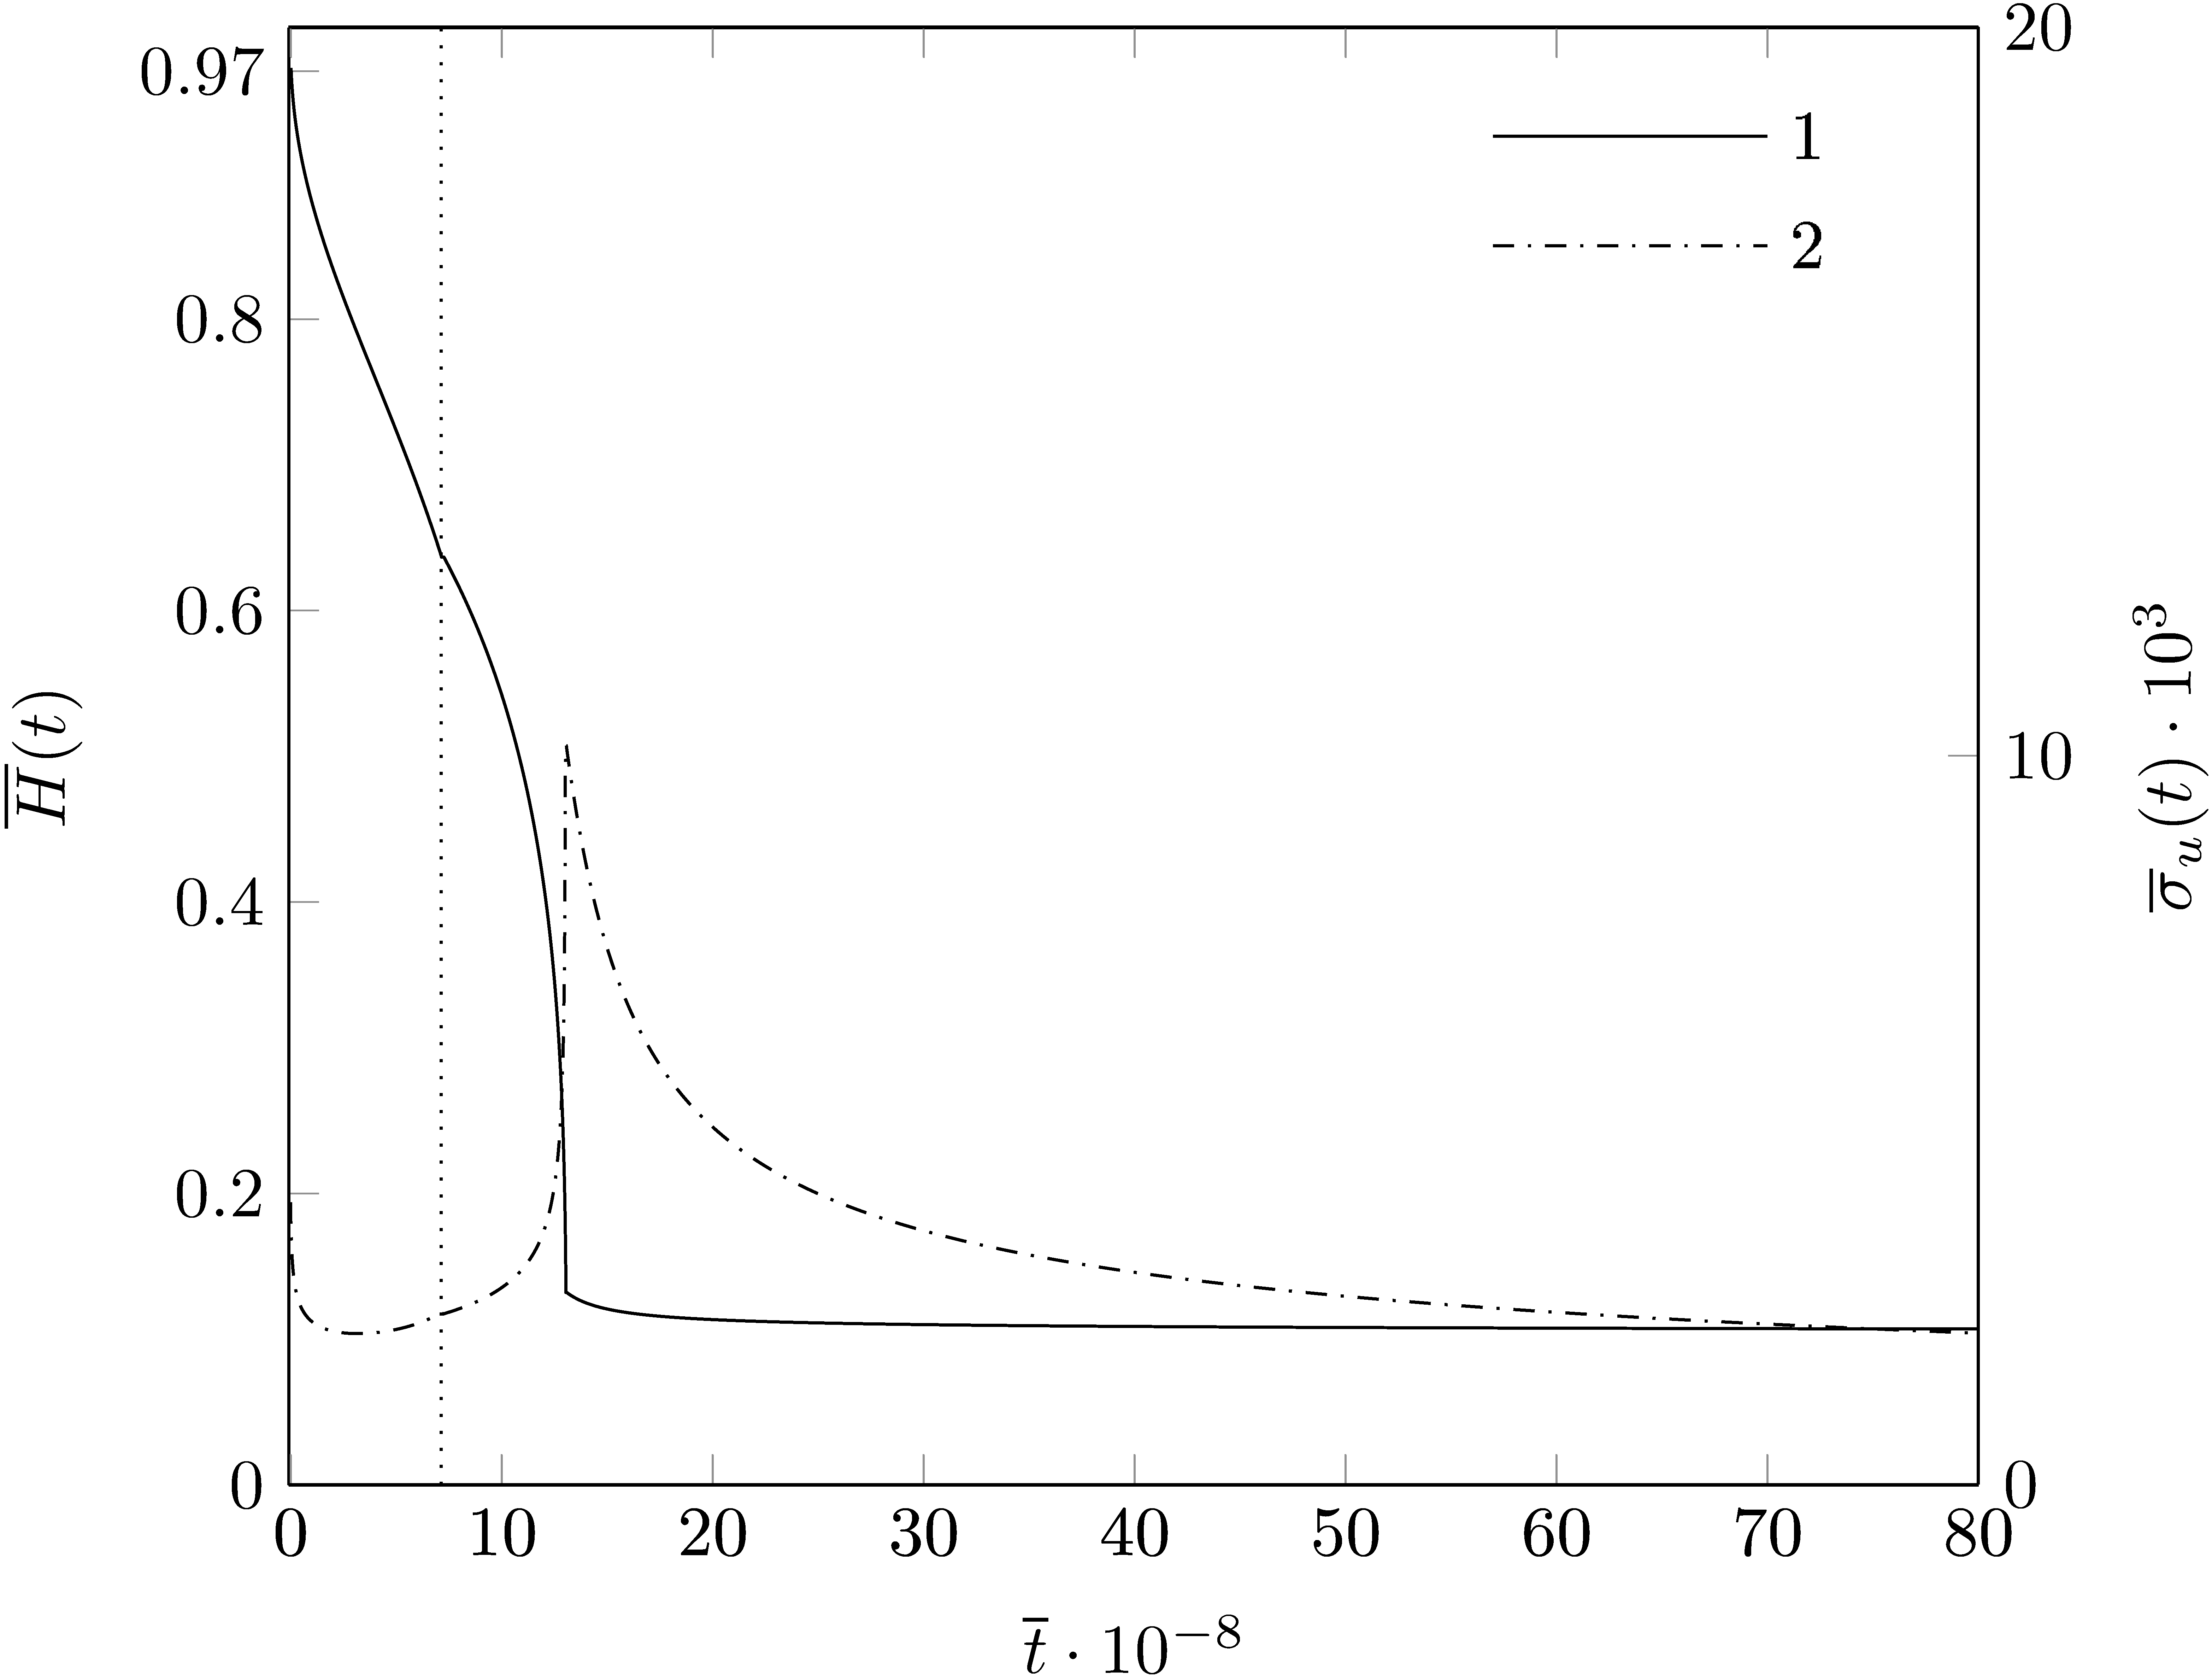
\includegraphics[width=0.8\linewidth]{images/ab7.png}}
				\caption{Зависимости толщины(1) и интенсивности напряжений(2) от времени при условии идеального скольжения внутри П-образной матрицы. Отношение $b/a = 7$} 
				\label{vert_sliging_7ba}
		\end{figure}
				\begin{figure}[h!]	
				\def\svgwidth{\columnwidth}
				\center{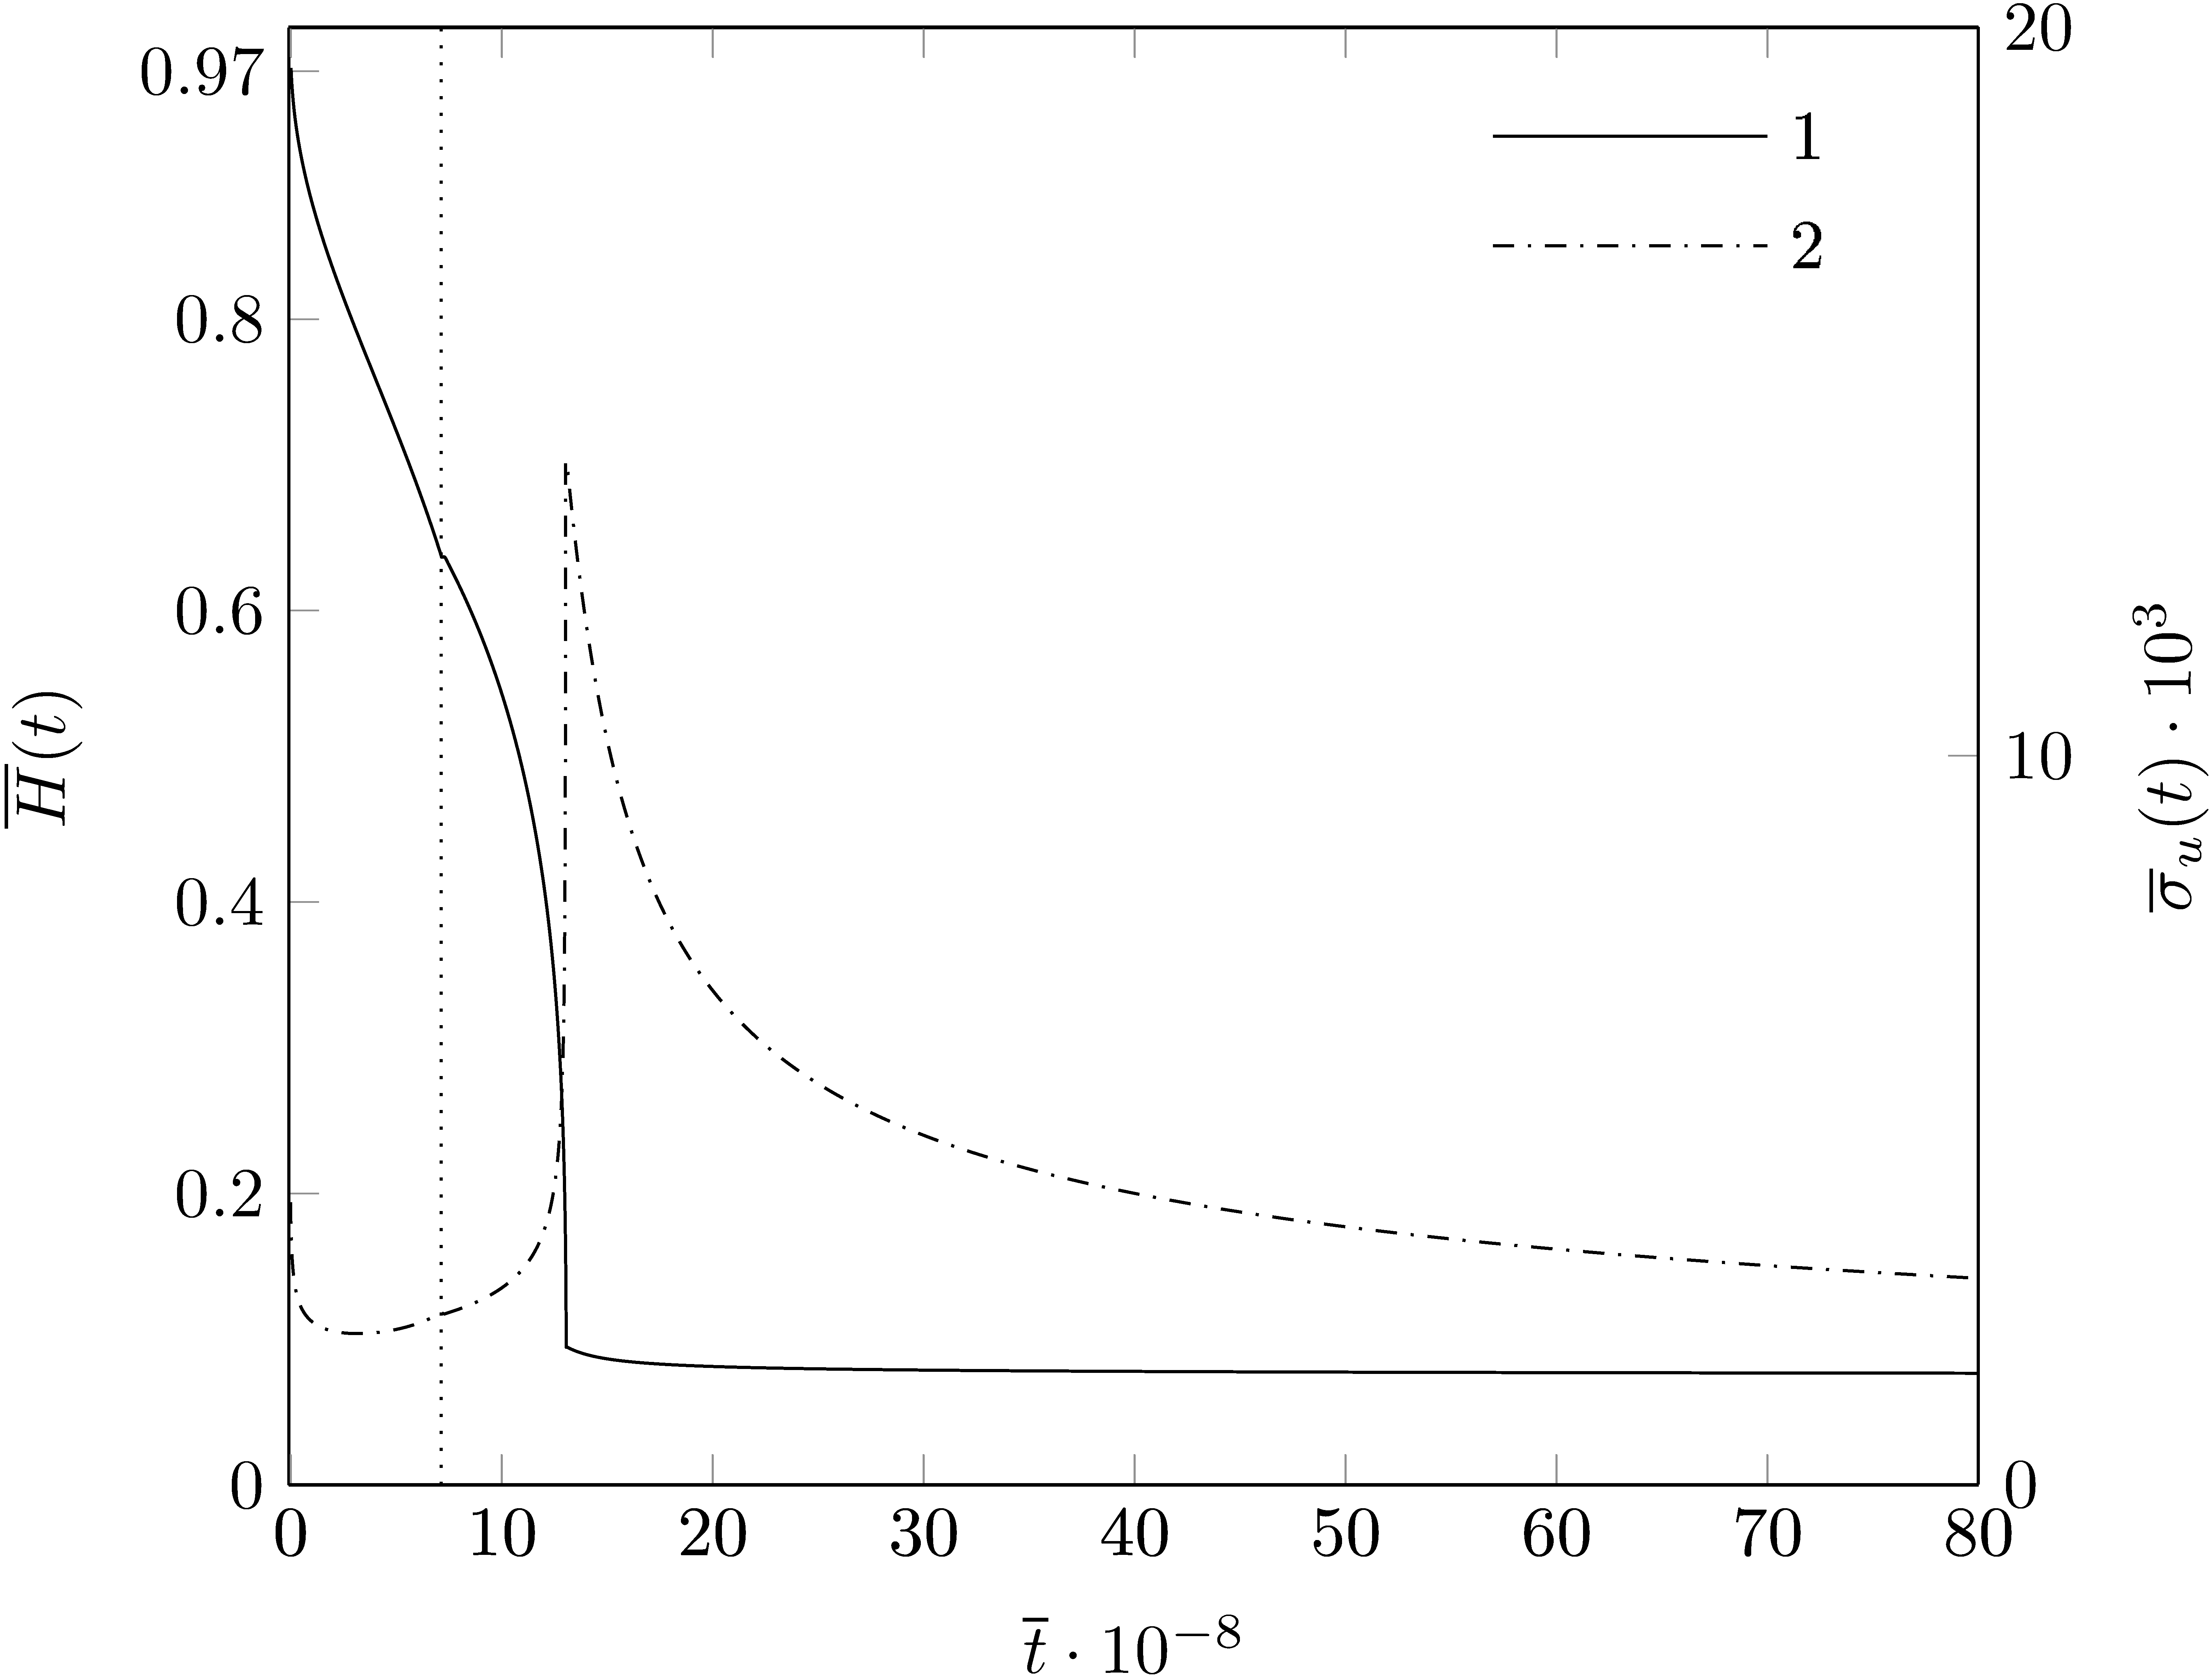
\includegraphics[width=0.8\linewidth]{images/ab10.png}}
				\caption{Зависимости толщины(1) и интенсивности напряжений(2) от времени при условии идеального скольжения внутри П-образной матрицы. Отношение $b/a$ = 10} 
				\label{vert_sliging_10ba}
		\end{figure}

Для другого граничного условия~--- прилипание мембраны к стенке матрицы~--- был проведен численный расчет и получены следующие результаты:
для \linebreak$b<10.8\cdot a$ происходит заполнение мембраны за бесконечное время. Для матриц у которых отношение высоты к ширине превосходит
10.8 раз наступает разрушение на третьем этапе деформации. Графики построены для случаев $b=a$, $b=4.5a$, $b=7a$, $b=10.8a$.
 
						 
		\begin{figure}[h!]	
				\def\svgwidth{\columnwidth}
				\center{\includegraphics[width=0.8\linewidth]{images/stick_ab.png}}
				\caption{Зависимости толщины(1) и интенсивности напряжений(2) от времени при условии прилипания внутри П-образной матрицы. Отношение $b/a = 1$} 
				\label{vert_stick_ba}
		\end{figure}

		\begin{figure}[h!]	
				\def\svgwidth{\columnwidth}
				\center{\includegraphics[width=0.8\linewidth]{images/stick_ab45.png}}
				\caption{Зависимости толщины(1) и интенсивности напряжений(2) от времени при условии прилипания внутри П-образной матрицы. Отношение $b/a = 4.5$} 
				\label{vert_stick_4ba}
		\end{figure}
				\begin{figure}[h!]	
				\def\svgwidth{\columnwidth}
				\center{\includegraphics[width=0.8\linewidth]{images/stick_ab7.png}}
				\caption{Зависимости толщины(1) и интенсивности напряжений(2) от времени при условии прилипания внутри П-образной матрицы. Отношение $b/a = 7$ }
				\label{vert_stick_7ba}
		\end{figure}
				\begin{figure}[h!]	
				\def\svgwidth{\columnwidth}
				\center{\includegraphics[width=0.8\linewidth]{images/stick_ab10.png}}
				\caption{Зависимости толщины(1) и интенсивности напряжений(2) от времени при условии прилипания внутри П-образной матрицы. Отношение $b/a = 10.8$} 
				\label{vert_stick_10ba}
		\end{figure}

\clearpage

\section{Анимирование}
\subsection{Используемые инструменты}
В качестве средства построения трех-мерного изображения было выбрано программное 
средство OpenGL. Оно представляет собой свободное программное обеспечение, состоящее 
из большого набора библиотек и простой процедурный интерфейс [\ref{opengl-manual}]. 
Несмотря на это с  помощью OpenGL можно создавать сложные и мощные программные 
комплексы, затрачивая при 
этом минимальное время по сравнению с другими графическими библиотеками. При этом с 
помощью OpenGL обеспечивается высокая эффективность работы с графическими объектами.
%а тут наверно тоже можно раздуть
\subsection{Подготовка выходных данных}
Изначально полученная зависимость имеет равномерный шаг по переменной $x$ и переменный по искомой $t$. Чтобы видео отражало реальную временную зависимость требуется перейти к равномерному шагу по $x$ и неравномерному по $t$.
Так же нужно было расширить выходные параметры значениями толщины. Для перехода к равномерному шагу по $t$ использовалась линеаризация значений, по следующему алгоритму:
\begin{itemize}
\item[1.] Найти среднее значение $\Delta t$,
\item[2.] Пересчитать зависимость $x(t)$, с шагом $\Delta t$:
\begin{itemize}
	\item[2.1] Если очередной отрезок $(x_k; x_{k+1})$ имеет шаг по $t$ больше, чем $\Delta t$, берем линейное приближение для вычисления $x_{k+1}(t_k+\Delta t)$, операция выполняется кратно отношению $\frac{t_{k+1}-t_k}{\Delta t}$,
	\item[2.2] Иначе выкидываем точку $x_{k+1}$ из новых выходных данных.
\end{itemize}
\end{itemize} 
Таким образом получаем усредненную и равномерную зависимость по времени, которую уже на вход получает модуль графической интерпретации данных. Ниже представлены различные 
кадры из видео деформирующейся мембраны.
		\begin{figure}[h!]	
				\def\svgwidth{\columnwidth}
				\center{\includegraphics[width=0.5\linewidth]{images/state11.png}}
				\caption{}				
				\label{animate1}
		\end{figure}

		\begin{figure}[h!]	
				\def\svgwidth{\columnwidth}
				\center{\includegraphics[width=0.5\linewidth]{images/state12.png}}
				\caption{} 
				\label{animation2}
		\end{figure}
				\begin{figure}[h!]	
				\def\svgwidth{\columnwidth}
				\center{\includegraphics[width=0.5\linewidth]{images/state21.png}}
				\caption{} 
				\label{animation3}
		\end{figure}
				\begin{figure}[h!]	
				\def\svgwidth{\columnwidth}
				\center{\includegraphics[width=0.5\linewidth]{images/state22.png}}
				\caption{} 
				\label{animation4}
		\end{figure}
		\begin{figure}[h!]	
				\def\svgwidth{\columnwidth}
				\center{\includegraphics[width=0.5\linewidth]{images/state33.png}}
				\caption{} 
				\label{animation5}
		\end{figure}
\clearpage
